%Num-Projekt1, Amanda ? , Christoph Mayer

\documentclass[a4paper,11pt,bibliography=totoc,listof=totoc,headinclude=true,cleardoublepage=empty,oneside]{scrbook}
% Option "oneside" für einseitigen Druck. Weglassen, falls die Arbeit doppelseitig gedruckt wird
\usepackage{graphicx} 
\usepackage[english,ngerman]{babel}
\usepackage[utf8]{inputenc}
%\usepackage{fullpage}
\usepackage{ifthen}
\usepackage{color}
\usepackage{amsmath,amsthm,amssymb,amsfonts}
\usepackage{graphicx}
\usepackage{amsmath}
\usepackage{mathtools}
\usepackage{tikz}
% links in pdf
\usepackage[unicode,colorlinks=true,pagebackref=false]{hyperref}
\usepackage{listings}
\usepackage{maplestd2e}
% Zum Druck verwende schwarze Links!
%\usepackage[unicode,colorlinks=true,linkcolor=black,citecolor=black,urlcolor=black,pagebackref=false]{hyperref} 
% colorlinks=false umrahmt Links statt einzufaerben, 


% document style
\KOMAoptions{footinclude=false} % Fusszeile wird nicht zu Satzspiegel gezaehlt
\KOMAoptions{headsepline=true} % Trennlinie zwischen Kopfzeile und Text
\KOMAoptions{DIV=12} % beeinflusst Satzspiegel
\KOMAoptions{BCOR=8mm} % Bindekorrektur
\pagestyle{headings} % mit Kopfzeilen

\recalctypearea % berechne Satzspiegel neu

\definecolor{change}{rgb}{0,.55,.55}



\def\revision#1{{\color{red}#1}}

%%%%%%%%%%%%%%%%%%%%%%%%%%%%%%%%%%%%%%%%%%%%%%%%%%%%%%%%%%%%%%%%%%%%%%%%%%%%%%%%%%%%%%%%%%%%%%%%%%%%%%%%%%%%%%
%%%%%%%%%%%%%%%%%%%%%%%%%%%%%%%%%%%%%%%%%%%%%%%%%%%%%%%%%%%%%%%%%%%%%%%%%%%%%%%%%%%%%%%%%%%%%%%%%%%%%%%%%%%%%%
%%%%%%%%%%%%%%%%%%%%%%%%%%%%%%%%%%%%%%%%%%%%%%%%%%%%%%%%%%%%%%%%%%%%%%%%%%%%%%%%%%%%%%%%%%%%%%%%%%%%%%%%%%%%%%
%%%%%%%%%%%%%%%%%%%%%%%%%%%%%%%%%%%%%%%%%%%%%%%%%%%%%%%%%%%%%%%%%%%%%%%%%%%%%%%%%%%%%%%%%%%%%%%%%%%%%%%%%%%%%%

\begin{document}


\pagenumbering{Alph}
\selectlanguage{ngerman}

\begin{titlepage}
	%\vspace*{-2cm}
	\begin{center}
	%	\includegraphics[width=0.45\textwidth]{TULogo.eps}
		\vskip 1cm%
		{\LARGE B~\Large N~U~M~E~R~I~R~K}
		\vskip 8mm
		{\huge\bfseries\color{change}Projekt 1}
		\vskip 1cm
		
		{\Large\bfseries\color{change}Name des Tutors: Johann Faschingleitner}\\[1ex]
		\vskip 0.5cm
		{\Large\bfseries\color{change}Name der Autoren:}\\[1ex]
		\vskip 0.5cm
		Christoph Mayer
		\vskip 0.5cm
		Matrikelnummer: {\color{change}e01425430}\\[1ex]
		\vskip 0.5cm
		Amanda
		\vskip 0.5cm
		Matrikelnummer: {\color{change}e01425430}\\[1ex]
	\end{center}
\end{titlepage}

\cleardoublepage
	
\chapter*{Aufgabe 3:} %\chapter*{Acknowledgement}
\thispagestyle{empty}
\selectlanguage{ngerman} %\selectlanguage{english}


{\color{change}
	\begin{itemize}
		\item 3.1 Basierend auf einer 1D Quadratur kann durch Bildung des Tensorproduktes eine 2D Quadratur erzeugt werden. Sei dazu $f:	\mathbb{R} ^2 \to \mathbb{R}$ eine auf dem Einheitsqudrat $Q:=
		%hier für intervalle was besonderes? bzw das x fürs produkt der intervalle nicht gut
		 [0,1]x[0,1]$ integrierbare Funktion, dann gilt (mittels Fubini):
		\begin{equation}
		
		\int \limits_{\^{Q}} \! f(x,y) \, d(x,y) = 
		\int_0^{1}(\int_0^{1}f(x,y)dx)dy=
		\int_0^{1}(\sum_{i=0}^n\alpha_i f(x_i,y))dy= \sum_{i=0}^n \alpha_i \int_0^{1} f(x_i,y)dy=
		\sum_{i=0}^{n} \alpha_i(\sum_{j=0}^{n} \alpha_j f(x_i,y_i))=
		= \sum_{i,j=0}^{n} \alpha_i\alpha_j f(x_i,y_j)
		%hier große klammern
		
		%begin{split}
		%a^2 &= b^2 + c^2 \\\
	%	&> b^2
	%	\end{split}
	%	\sum_{j=1}^n j = \frac{n(n+1)}{2}
s 		\end{equation}

		wobei $ \{\alpha_i =0,...n\} $  und  $\{x_i,y_i : i=0,...n\}$ die 1D Quadraturgewichte und -knoten sind- Somit kann man mit den bereits bekannte 1D Quadraturen auch Integrale am Einheitsquadrat numerisch berechnen. Implementieren Sie mit Hilfe des zur Verfügung gestellten Programms \textbf{gauss(n)} eine Funktion \textbf{quadInt(f,n)} die $\int \limits_{\^{Q}} \! f(x,y) \, d(x,y) $ berechnet. Für welche n wird ein Polynom $ p \in \prod_{2}^k:=span\{x^iy^j:0 \leq i,j\leq k \} $ exakt integriert?
		
		
		 
		\lstset{ 
			language=Matlab, 
			showstringspaces=false}
	
		\lstinputlisting{quadInt.m} 
		\begin{lstlisting} 
		

		\end{lstlisting}
		
		Plot:
	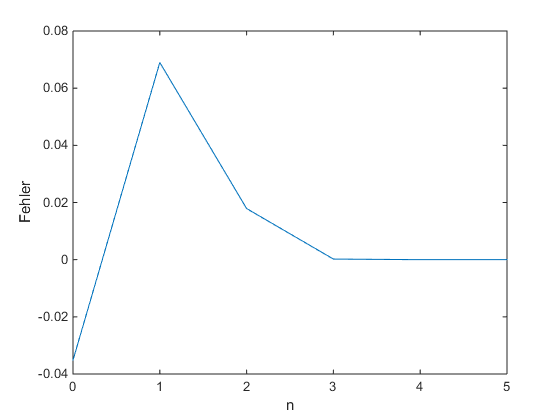
\includegraphics[width=0.7\textwidth]{plot1.png} %70% der Textbreite
	\begin{figure}
		\centering
		\includegraphics[width=0.7\textwidth]{"plot1.png"}
		\caption{Erstes Bild}
		\label{fig:Bild1}
	\end{figure}
		# Die Aufgabennummerierung in Absätzen, als 3.1 unter 3.2 etc. und Text daneben
		
		Widmen wir uns jetzt noch der Frage für welche n ein Polynom $ p \in \prod_{2}^k:=span\{x^iy^j:0 \leq i,j\leq k \} $ exakt integriert wird:
		
		Wir wissen dass für 1D Quadraturen Polynome vom Grad 2n+1 exakt numerisch berechnet werden können. Da in (0.1) lediglich die Gauß-Quadratur 2-mal hintereinander eindimensional durchgeführt wird, gilt, dass i=2n+1 und j=2n+1 die höchsten Grade sind, für welche die 2D Quadratur exakt numerisch berechnet werden kann.
		
		
		\item 3.2 Da zum Beispiel bei der Finite-Element-Methode eine Quadratur auf Dreiecken benötigt wird, verwendet man gerne die \texit{Duffy-Transofrmation} um die Quadratur auf dem Einheitsquadrat \^{Q} auf das Referenzdreieck \^{T} mit den Eckpunkten $ (0,0),(1,0)$ und $ (0,1)$ zu transformieren.
		Die \texit{Duffy-Transformation} ist definiert als:
		
		\begin{equation} 
		\PSI = \begin{cases} 
		\^{Q} \to \^{T} \\
		(s,t) \mapsto (s,(1-s)t)
		\end{cases} 
		\end{equation} 
		
		Implementieren Sie mithilfe der \textit{Duffy-Transformation} die Funktion \textbf{trigInt(f,n)}, sodass Sie Integrale auf \^{T} berechnen können.
		\textit{Hinweis}: Verwenden Sie dazu die Substitutionsregel Satz 7.34 (Transformationssatz für Integrale) aus dem Analysis-Skript von Professor Engl.
		
		Transformationssatz für Integrale:
		
		Es sei $\Omega \in \mathbb{R}$ eine offene Menge und $\Phi:\Omega \to \Phi(\Omega) \in \Mathbb{R}^d$ ein Diffeomorphismus. Dann ist die Funktion $f$ auf $\Phi(\Omega)$ genau dann integrierbar, wenn die Funktion $x \mapsto f(\Phi(x)) |det(D\Phi(x))| $ auf $\Omega$ integrierbar ist.
		In diesem Fall gilt:
		
		$\int_{\Phi(\Omega)}^{}f(y)dy = \int_{\Omega}f(\Phi(x))|det(D\Phi(x))|dx.$
		
		Dabei ist $D\Phi(x)$ die Jacobi-Matrix und $det(D\Phi(x))$ die Funktionaldeterminante  von $\Phi$.
		
		DEF FUNKTIONALDETERMINANTE
		
		Auf unseren Fall mit $\Omega=\^{Q}$, $\Psi=\^{T}$, sowie mit der Funktionaldeterminante 
		
			$ det D\^{T} = |det		
			\left(
			\begin{array}{ccc}
			1 & -t \\
			0 & (1-s)\\
			\end{array}
			\right)| = |(1-s)| $
			
			ergibt sich:
			
		$	\int_{\^{T}}^{}f(x,y)d(x,y) = \int_{\^{Q}}^{}f(s,(1-s)t)|(1-s)|d(t,s)
			= \sum_{{i,j=0}}^{n}\alpha_i \alpha_j f(s_i,(1-s_i)t_j)|(1-s_i)| $
		
		
		Dadurch ergibt sich insgesamt:
		
		$trigInt(f,n) = quadInt(f\circ(s,t) \mapsto (s,(1-s)t))*(1-s)$
		
		\\[12pt]
		
		Implementierung von quadInt(f,n):
		\lstset{ 
			language=Matlab, 
			showstringspaces=false}
		
		\lstinputlisting{trigInt.m} 
		\begin{lstlisting} 
		
		
		\end{lstlisting}
		
		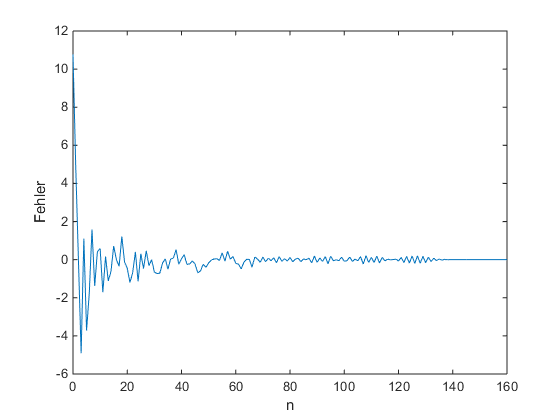
\includegraphics[width=0.7\textwidth]{plot2.png} %70% der Textbreite
		\begin{figure}
			\centering
			\includegraphics[width=0.7\textwidth]{"plot2.png"}
			\caption{Erstes Bild}
			\label{fig:Bild1}
		\end{figure}
		
		
		\item 3.3 Erweitern Sie unter Verwendung einer affinen Transformation $ \Phi_T:\^{T} \to T$ Ihre Implementierung von \textbf{duffyInt}, um auch Integralen auf beliebigen Dreiecken T berechnen zu können. 
		Für welche n wird ein Polynom $ p \in \prod_{2}^k:=span\{x^iy^j:0 \leq i+j\leq k \} $ exakt integriert? \\
		\textit{Hinweis:} Sie können die Implementation Ihrer Transformation testen, indem Sie das Integral über $f \equiv1$ numerisch berechnen und mit der analytisch bestimmten Fläche des Dreiecks T vergleichen
		
		Anstatt einer affinen Transformation von $ \Phi_\^{T}:\^{T} \to T$ verwenden wir eine (direkte?) affine Transformation $\Phi:\^{Q} \mapsto T$.
		
		Wir nehmen nun ein beliebiges Dreieck T mit $a=\left(
		\begin{array}{ccc}
		a_1 \\
		a_2\\
		\end{array}
		\right)$, $a=\left(
		\begin{array}{ccc}
			b_1 \\
			b_2\\
		\end{array}
		\right)$, $c=\left(
		\begin{array}{ccc}
			c_1 \\
			c_2\\
		\end{array}
		\right)$, 
		
		v=$\left(
		\begin{array}{ccc}
		(1-s)*a_1+ s*c_1\\
		(1-s)*a_2+s*c_2\\
		\end{array}
		\right)$ 	und w=$\left(
		\begin{array}{ccc}
			(1-s)*b_1+ s*c_1\\
			(1-s)*b_2+s*c_2\\
		\end{array}
		\right)$
		
		zur Hand, wobei die Vekotren $v$ und $w$ Konvex-Kombinationen der Punkte $a$ und $b$ sind:
		
		
		\begin{tikzpicture}[>/.tip=Latex, auto=right] 
		%Koordinaten für die Beschriftung 
		\coordinate[label=left:$a$]  (A) at (0,0); 
		\coordinate[label=right:$b$] (B) at (5,2); 
		\coordinate[label=above:$c$] (C) at (1,2.5); 
		
		\draw (A) -- (B) -- (C) -- (A);
		\path [->] 
		(A) edge node [left]{$\vec{v}$} (C)   
		(B) edge node {$\vec{w}$} (C)   
		; 
		\end{tikzpicture}
	
	
		Das (aus 3.2 oder bereits transformiert) Dreieck kann nun wie folgt dargestellt werden:
			$(1-t)v+s*w)$
			
		und die angepasste \textit{Duffy-Transformation} lautet wie folgt:
		
			$(s,t) \mapsto \left(
			\begin{array}{ccc}
				a_1 + s*(c_1-a_1)+ t*(b_1-a_1) + st(a_1-b_1)\\
				a_2 + s(c_2-a_2) + t(b_2-a_2) + st(a_2-b_2)\\
			\end{array}
			\right)$.
			
		Durch Proberechnung anhand des Beispiel unseres Referenzdreiecks, mit $a=\left(
		\begin{array}{ccc}
		0 \\
		0\\
		\end{array}
		\right)$, $a=\left(
		\begin{array}{ccc}
		0 \\
		1\\
		\end{array}
		\right)$, $c=\left(
		\begin{array}{ccc}
		1\\
		0\\
		\end{array}
		\right)$, folgt:
		
		\begin{tikzpicture}[>/.tip=Latex, auto=right] 
		%Koordinaten für die Beschriftung 
		\coordinate[label=left:$a$]  (A) at (0,0); 
		\coordinate[label=right:$b$] (B) at (0,3); 
		\coordinate[label=above:$c$] (C) at (3,0); 
		
		\draw (C) -- (B) -- (A) -- (C)
		 
	 
		; 
		\end{tikzpicture}
		
		$(s,t) \mapsto  c=\left(
		\begin{array}{ccc}
			t-st\\
			s\\
		\end{array}
		\right) = \left(
		\begin{array}{ccc}
			t*(1-s)\\
			s\\
		\end{array}
		\right)$
	
	
		Damit ist unsere Transformation korrekt und wir können uns an das Implementieren des Codes wagen:
		
		\lstset{ 
			language=Matlab, 
			showstringspaces=false}
		
		
		
		\lstinputlisting{duffyInt.m} 
		\begin{lstlisting} 
		
		
		\end{lstlisting}
		
		
		Widmen wir uns nun noch der Frage wann ein Polynom $ p \in \prod_{2}^k:=span\{x^iy^j:0 \leq i+j\leq k \} $ exakt integriert werden kann:
		
		Da wir nur die Hülle $span{x^iy^j:0 \leq i+j \leq k}$ betrachten können wir das Polynom $p=x^iy^j$ mit den höchstmöglichen Graden $i$ und $j$ heranziehen.
		
		Sei nun $ p \in \prod_{2}^k \Rightarrow \int_{\^{T}}^{} p(x,y)d(x,y) = 
		\int_{\^{Q}}^{} p(\Phi(x),\Phi(y)) * det|d\Phi| d(s,t)$ .
		
		Für $p=x^iy^j"$ lautet die Transformation wie folgt:
		
		$p(\Phi(x),\Phi(y)) = (\alpha_1+s\alpha_2+t\alpha_3+st\alpha_4)^i(\beta_1+s\beta_2+t\beta_3+st\beta_4)^j$.
			
			Aus diesem Ausdruck lesen wir heraus dass der höchste Term 
			
			$\delta_0s^it^is^jt^j = s^(i+j)t^(i+j)\delta_0$
			
			mit einer Konstanten $\delta_0$ die in diesem Fall vernachlässigt werden kann.
			
			Hingegen ist der höchste Term der Funktionaldeterminante $det|D\Phi|$:
			
			$\delta_1st$
			KORRIGIEREN, schöner SCHREIBEN
			WO FEHLT OBEN DIE TRANSFORMATION BEI DER DIE FUNKTIONALDETERMINANTE NOCH ANGEHÄNGT WERDEN MUSS
			
			Somit ist der größte Term von
			 $\int_{\^{Q}}^{} p(\Phi(x),\Phi(y)) * det|d\Phi| d(s,t)$ 
			 vom Grad
			 $\deltas^{i+j+1}t^{i+j+1}$.
			 Da $i+j+1\leq2n+1$ gefordert wird, ergibt sich $i+j\leq2n$.
			 			
			
		

		
		\item 3.4 Erweitern Sie Ihre Implementierung von \textbf{[quadInt(f,n)} zur Berechnung von Integralen auf beliebigen konvexen Vierecken $ Q=conv{(a1,a2),(b1,b2),(c1,c2),(d1,d2)} $. Verwenden Sie dazu eine eine Transformation der Form:
		
			\begin{equation} 
			\Psi_{\^{Q}} = \begin{cases} 
			\^{Q} \to Q \\
			(u,v) \mapsto
			
		 \left(
		  \begin{array}{ccc}
		  \alpha_1 + \alpha_{2}u + \alpha_{3}v +\alpha_{4}uv \\
		  \beta_1+\beta_{2}u+beta_{3}v+\beta_{4}uv \\
		  \end{array}
		  \right)

			\end{cases} 
			\end{equation} 
			
		mit den Konstanten $\alpha_i,\beta_i \in \mathebb{R}$. Überlegen Sie sich, warum nicht-konvexe Vierecke unzulässig sind.
		
		
		\lstset{ 
			language=Matlab, 
			showstringspaces=false}
		
		\lstinputlisting{quadInt2.m} 
		\begin{lstlisting} 
		
		
		\end{lstlisting}
		
		
		
		\begin{figure}
			\centering
			\includegraphics[width=0.7\textwidth]{"plot4.png"}
			\caption{Erstes Bild}
			\label{fig:Bild1}
		\end{figure}
		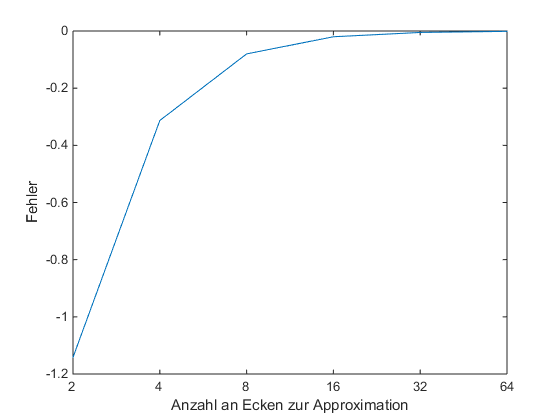
\includegraphics[width=0.7\textwidth]{plot4.png} %70% der Textbreite
		
		
		
		\item 3.5 Testen Sie ihre Quadraturen für \int \limits_{G} \! f(x,y) \, d(x,y):
		
		\par
		\begingroup
		\leftskip=1cm % Parameter anpassen
		\noindent %ab hier der Text, der eingerückt werden soll
		\begin{itemize}
				
			\item $f(x,y)= x^7+3x^4y^4+3x^2y+7y^6 , G=conv\{(0,0),(0,5,-0,5),(1,1)\}$ \\
			Stimmt das benötigte n um das Prolynom exakt zu integrieren mit den theoretischen Überlegen zusammen? Wenn nicht, wieso?
			
				\lstset{ 
					language=Matlab, 
					showstringspaces=false}
				
				\lstinputlisting{aufg3_5_1.m} 
				\begin{lstlisting} 
				
				
				\end{lstlisting}
				
			
			\item $f(x,y)=\sin(50x)\sin(50y), G=conv\{(1,0),(10.2),(3,4)(-1,1)\})$
				\lstset{ 
					language=Matlab, 
					showstringspaces=false}
				
				\lstinputlisting{aufg3_5_2.m} 
				\begin{lstlisting} 
				
				
				\end{lstlisting}			

			\item $f(x,y)= \sqrt{\frac{9y}{(1-x^2)}} , G=\^{Q} $

				\lstset{ 
					language=Matlab, 
					showstringspaces=false}
				
				\lstinputlisting{aufg3_5_3.m} 
				\begin{lstlisting} 
				
				
				\end{lstlisting}			
			\item
					$ f(x,y) = \begin{cases} 
					1, x^2+y^2 \leq 1 \\
					0, sonst
					\end{cases} , G=\mathbb{R}^2$
					
				\lstset{ 
					language=Matlab, 
					showstringspaces=false}
				
				\lstinputlisting{aufg3_5_4.m} 
				\begin{lstlisting} 
				
				
				\end{lstlisting}
				
		\end{itemize}		
		
		\textit{Hinweis:} Approximieren Sie den Kreis durch ein n-Eck.
		Verwenden Sie die letzten beiden Beispiele um $\pi$ zu approximieren.
		Nehmen Sie als Referenzwert bei allen Integralen den analytisch bestimmten Integralwert, sofern dies mölgich ist und stellen Sie die Fehler grafisch dar.
		\par
		\endgroup		
	
	
		
	
			 
		
		
		\end{itemize}
		
	\end{itemize}
}

\end{document}